\makeatletter
\def\@makechapterhead#1{%
  \vspace*{10\p@}%
  {\parindent \z@ \raggedleft \normalfont
    \ifnum \c@secnumdepth >\m@ne
      \if@mainmatter
        \LARGE\bfseries \@chapapp\space \thechapter
	\vskip 4pt
        \hrule height 2pt
        \par\nobreak
        \vskip 5\p@
      \fi
    \fi
    \interlinepenalty\@M
    \huge \bfseries #1\par\nobreak
\vskip 5pt

\hrule height 2pt   
 \vskip 10\p@  
  }}
\makeatother

\chapter{Bipolar Junction Transistor}\label{chap2}
\addtocontents{toc}{\protect\contentsline{chapter}{\protect Chapter \numberline{\thechapter.}
  Bipolar Junction Transistor}{\thepage--\pageref{2end}}}  

\medskip
\section{Junction Transistor}\label{sec2.1}

The bipolar junction transistor (BJT) is simply a sandwich of one type of semiconductor material (p-type or n-type) between two layers of the other type. If a layer of n-type material is sandwiched between two layers of p-type as shown in Fig.~\ref{fig2.1}(a), it is called {\em pnp transistor}. Similarly, if a layer of p-type material is sandwiched between two layers of n-type as shown in Fig.~\ref{fig2.1}(b), it is called an {\em npn transistor}.
\begin{figure}[H]
\centering
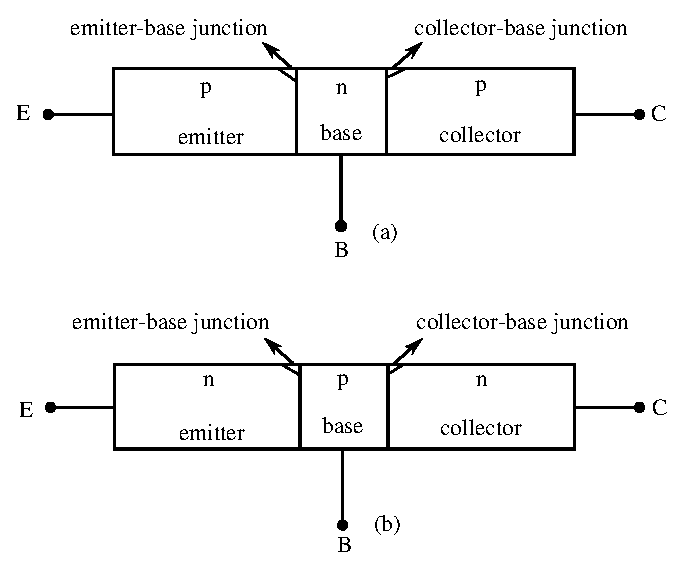
\includegraphics{chap2/fig1.eps}
\caption{(a) pnp transistor~~~ (b) npn transistor}\label{fig2.1}
\end{figure}

The center layer is called the {\em base}, one of the outer layer is called the {\em emitter} and the other outer layer is called the {\em collector}. The layers of emitter, base and collector are provided with terminals which are appropriately labelled E, B and C respectively. Two pn junction exist within each transistor; the emitter-base junction and the collector-base junction.

The base region is lightly doped and very thin compared to the heavily doped emitter and the moderately doped collector region.

Fig.~\ref{fig2.2} shows the schematic symbols for an npn and a pnp bipolar junction transistors. The term bipolar corresponds to the use of both holes and electrons as carriers in the transistor. The arrow on the emitter shows the direction of conventional current flow in the transistor. In an npn transistor, arrow points outward and that in pnp transistor it points inward as shown in Fig.~\ref{fig2.2}.
\begin{figure}[H]
\centering
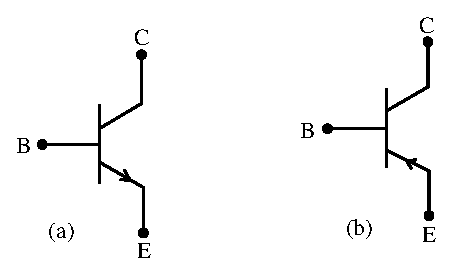
\includegraphics{chap2/fig2.eps}
\caption{(a) npn transistor~~~ (b) pnp transistor}\label{fig2.2}
\end{figure}

\medskip
\subsection{Basic transistor operation}\label{sec2.1.1}

The basic operation of a transistor will now be described using an npn transistor. This explanation is equally applicable to pnp transistor and can be translated for pnp transistor simply by interchanging the roles played by electrons and holes and reversing each voltage polarity.

Fig.~\ref{fig2.3} shows the correct bias for each junction in an npn transistor seperately, but in practice both junctions will be biased simultaneously. In Fig.~\ref{fig2.3}(a), the emitter-base junction is forward biased by a dc source labelled $\rmV_{\rmE\rmE}$. The negative terminal of $\rmV_{\rmE\rmE}$ is connected to $\rmn$ side of pn junction as required for forward bias. Consequently, there is a substantial flow of diffusion current across the junction due to the flow of majority carriers (i.e. electrons) from the n-type emitter. The depletion region at this junction is made narrow by the forward bias. Since the p-type base is very thin and has a low conductivity (because it is lightly doped), a very small number of these electrons will take path to the base terminal.

The magnitude of the base current is typically on the order of microamperes as compared to milliamperes for the emitter and collector currents. When the majority electrons diffuse into the base, they become minority carriers in that p-type base region. We say that minority carriers have been injected into the base.
\begin{figure}[H]
\centering
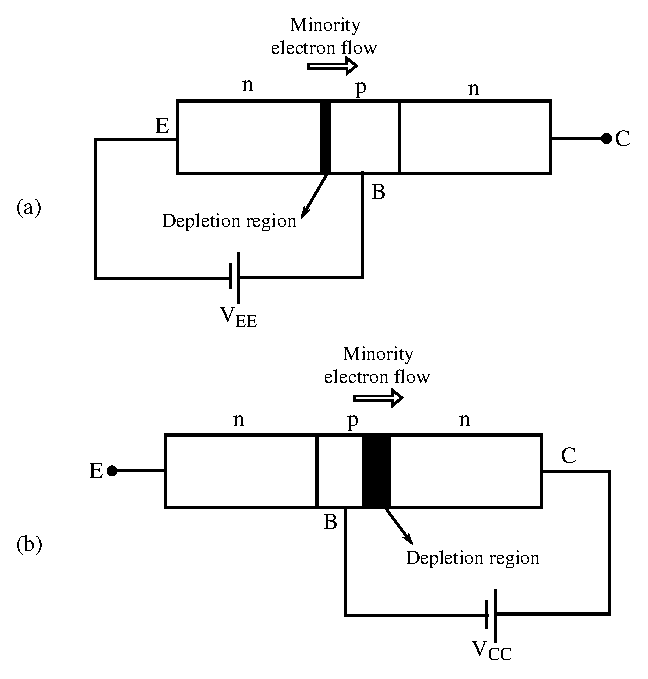
\includegraphics[scale=.95]{chap2/fig3.eps}
\caption{(a) Forward biasing emitter-base junction\\ (b) Reverse biasing collector-base junction}\label{fig2.3}
\end{figure}

Fig.~\ref{fig2.3}(b) shows that the collector-base junction is reverse biased by a dc source labelled $\rmV_{\rmC\rmC}$. The positive terminal of $\rmV_{\rmC\rmC}$ is connected to the n-type collector. Consequently, the depletion region at this junction is widened and the only current that flows from base to collector is due to the minority electrons crossing the junction from the p-type base, because the minority carriers readily cross a reverse biased junction.

Fir.~\ref{fig2.4} shows an npn transistor which is biased for normal operation with dc sources $\rmV_{\rmE\rmE}$ and $\rmV_{\rmC\rmC}$ connected simultaneously. The base is a common point or ground of the circuit and can therefore be regarded as being at zero volts. The emitter is negative with respect the base and the collector is positive with respect to the base. These are the conditions required to forward bias the emitter-base junction and to reverse bias the collector-base junction.
\begin{figure}[H]
\centering
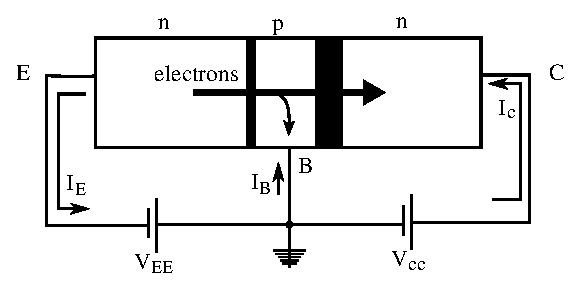
\includegraphics[scale=.97]{chap2/fig4.eps}
\caption{An npn transistor with emitter-base junction forward biased and collector-base junction reverse biased}\label{fig2.4}
\end{figure}
Since the base region is very thin and lightly doped, there are relatively few holes in it. So very few of the electrons injected into the base from the emitter recombine with holes. Instead, majority of the injected electrons into the base region diffuse to the reverse biased collector-base junction and swept across the junction. Since the electrons injected into the base will become minority carriers, there it will readily cross the reverse biased junction. Thus, the electron flow constitutes the dominant current type in an npn transistor. Similarly, for a pnp transistor hole current is dominant type.

Despite the fact that, most of the electrons injected into the base region cross into the collector, a few of them do combine with holes in the base. For each electron that combine with a hole, an electron leaves the base region via the base terminal. This action results in a very small base current which is about 2\%\ or less of the electron current from emitter to collector.

Fig.~\ref{fig2.4} also shows the arrows that are drawn to indicate the direction of conventional current in an npn transistor. Note that each arrow points in the opposite direction of the electron flow. Conventional current flowing through the collector is called {\em collector current} $\rmI_{\rmC}$, current through the base is called {\em base current} $\rmI_{\rmB}$ and current flowing through the emitter is called {\em emitter current} $\rmI_{\rmE}$.

Fig.~\ref{fig2.5}(a) and (b) shows a circuit diagram of an npn transistor and a pnp transistor respectively, with proper biasing for normal operation.


Observe that the emitter of an npn transistor has an arrow pointing out from the base whereas that of a pnp transistor shows an arrow pointing into the base. This arrow indicates the direction of conventional emitter current.

Applying Kirchoff's current law to the transistor of Fig.~\ref{fig2.5}, we obtain
\begin{equation}
\rmI_{\rmE}=\rmI_{\rmC}+\rmI_{\rmB}\label{eq2.1}
\end{equation}

\vfill\eject

\begin{figure}[H]
\centering
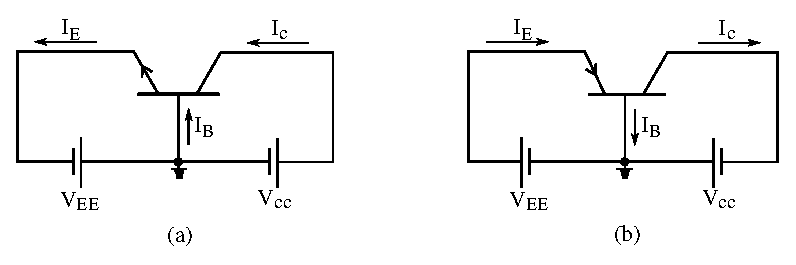
\includegraphics{chap2/fig5.eps}
\caption{(a) An npn transistor with proper biasing\\ (b) A pnp transistor with proper biasing}\label{fig2.5}
\end{figure}

\noindent
i.e., the emitter current is the sum of the collector current and the base current. However, the collector current is comprised of two components. One is due to the injected minority carriers into the base from the emitter and the other is due to the thermally generated minority carriers. We know that when a pn junction is reverse biased, there flows a small reverse current due to the thermally generated minority carriers. The direction of this small thermally generated collector current and the collector current due to the injected minority carriers are same and they get added up.
\begin{equation}
\text{i.e.,}\qquad \rmI_{\rmC}=\rmI_{\rmC(\text{inj})}+\rmI_{\text{CBO}}\label{eq2.2}
\end{equation}
where $\rmI_{C(\text{inj})}$ is the component of collector current due to injected minority carriers into the base from emitter and $\rmI_{\text{CBO}}$ is collector to base reverse current.


Eqn.~\eqref{eq2.2} can be written as
\begin{equation}
\rmI_{\rmC}=\alpha_{\text{dc}}\rmI_{\rmE}+\rmI_{\text{CBO}}\label{eq2.3}
\end{equation}

In Eqn.~\eqref{eq2.3}, $\alpha_{\text{dc}}$ indicates the portion of emitter current that survives after passage through the base to become collector current. Obviously, $\alpha_{\text{dc}}$ will be always less than 1 because some of the emitter current is drained off in the base through recombination. Typical transistors have values of $\alpha_{\text{dc}}$ that range from 0.95 to 0.995.

Since $\rmI_{\text{CBO}}$ is negligibly small in most practical situations, Eqn.~\eqref{eq2.3} can be written as
\begin{align}
\rmI_{\rmc} &\simeq \alpha_{\text{dc}}\rmI_{\rmE}\label{eq2.4}\\[4pt]
\therefore\quad \alpha_{\text{dc}} &= \frac{\rmI_{\rmC}}{\rmI_{\rmE}}\label{eq2.5}
\end{align}

Therefore, $\alpha_{\text{dc}}$ is approximately the ratio of collector current $\rmI_{\rmC}$ to emitter current $\rmI_{\rmE}$. $\alpha_{\text{dc}}$ is also referred to as {\em common base dc current gain}.

\section{Transistor Current Components}\label{sec2.2}

The various currents which flow within an npn transistor are shown in Fig.~\ref{fig2.6}.
\begin{figure}[H]
\centering
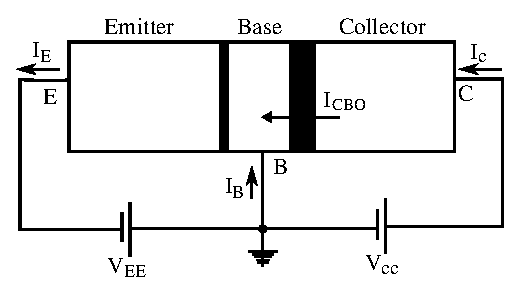
\includegraphics{chap2/fig6.eps}
\caption{Currents in an npn transistor}\label{fig2.6}
\end{figure}

$\rmI_{\rmE}$ is the emitter current. In an npn transistor, $\rmI_{\rmE}$ is a flow of electrons from the emitter to the base. $\rmI_{\text{CBO}}$ is a very small collector to-base leakage current due to thermally generated minority charge carriers flowing across the reverse biased collector-base junction. $\rmI_{\text{CBO}}$ is completely independent of all other currents. Even when the other currents are zero, $\rmI_{\text{CBO}}$ continues to flow when the collector-base junction is reverse biased.

$\rmI_{\rmB}$ is the base current, which is that portion of $\rmI_{\rmE}$ that flows in through the base terminal minus the value of $\rmI_{\text{CBO}}$. $\rmI_{\rmC}$ is the collector current, which is that portion of $\rmI_{\rmE}$ which flows across the collector-base junction with the addition of $\rmI_{\text{CBO}}$. Fig.~\ref{fig2.6} shows that $\rmI_{\rmE}$ flow outward of the transistor and that both $\rmI_{\rmB}$ and $\rmI_{\rmC}$ flow into the transistor.

So, we have
\begin{align}
\rmI_{\rmE} &= \rmI_{\rmC}+\rmI_{\rmB}\label{eq2.6}\\[4pt]
\text{and}\qquad \rmI_{\rmC} &= \alpha_{\text{dc}}\rmI_{\rmE}+\rmI_{\text{CBO}}\label{eq2.7}
\end{align}

Typical value of $\alpha_{\text{dc}}$ ranges from 0.95 to 0.995.

From Eqn.~\eqref{eq2.7}, we have,
\begin{equation}
\alpha_{\text{dc}} = \frac{\rmI_{\rmC}-\rmI_{\text{CBO}}}{\rmI_{\rmE}}\label{eq2.8}
\end{equation}

Since $\rmI_{\text{CBO}}$ is very much smaller than $\rmI_{\rmC}$, we have,
\begin{equation}
\alpha_{\text{dc}}\simeq \frac{\rmI_{\rmC}}{\rmI_{\rmE}}\label{eq2.9}
\end{equation}

Therefore, $\alpha_{\text{dc}}$ is approximately the ratio of collector current to emitter current. $\alpha_{\text{dc}}$ is also referred to as {\em common-base dc current gain}.

Substituting Eqn.~\eqref{eq2.6} in Eqn.~\eqref{eq2.7}, we get,
\begin{align}
& \rmI_{\rmC}=\alpha_{\text{dc}}(\rmI_{\rmC}+\rmI_{\rmB})+\rmI_{\text{CBO}}\notag\\[4pt]
& \rmI_{\rmC}(1-\alpha_{\text{dc}})=\alpha_{\text{dc}}\rmI_{\rmB}+\rmI_{\text{CBO}}\notag\\[4pt]
\therefore\quad \rmI_{\rmC} &= \dfrac{\alpha_{\text{dc}}}{1-\alpha_{\text{dc}}}\cdot \rmI_{\rmB}+\frac{1}{(1-\alpha_{\text{dc}})}\cdot \rmI_{\text{CBO}}\label{eq2.10}\\[4pt]
\rmI_{\rmC} &= \beta_{\text{dc}}\rmI_{\rmB}+(\beta_{\text{dc}}+1)\rmI_{\text{CBO}}\label{eq2.11}\\[4pt]
\text{where}\quad \beta_{\text{dc}} &= \frac{\alpha_{\text{dc}}}{1-\alpha_{\text{dc}}}
\end{align}
Since $\rmI_{\text{CBO}}$ is very much smaller than $\rmI_{\rmB}$, Eqn.~\eqref{eq2.11} can be written as
\begin{align}
\rmI_{\rmC} &\simeq \beta_{\text{dc}}\rmI_{\rmB}\label{eq2.12}\\[4pt]
\therefore\quad \beta_{\text{dc}} &\simeq \dfrac{\rmI_{\rmC}}{\rmI_{\rmB}}\label{eq2.13}
\end{align}

Thus, $\beta_{\text{dc}}$ is approximately the ratio of collector current to base current. $\beta_{\text{dc}}$ is also referred to as {\em common emitter dc current gain}. Typical value of $\beta_{\text{dc}}$ ranges from 20 to 2000 or higher.

The relationship between $\alpha_{\text{dc}}$ and $\beta_{\text{dc}}$ can also be obtained as below.

We have,
\begin{equation}
\rmI_{\rmE}=\rmI_{\rmC}+\rmI_{\rmB}\label{eq2.14}
\end{equation}

Dividing by $\rmI_{\rmC}$ on both the sides, we get
\begin{equation}
\frac{\rmI_{\rmE}}{\rmI_{\rmC}}=\frac{\rmI_{\rmC}}{\rmI_{\rmC}}+\frac{\rmI_{\rmB}}{\rmI_{\rmC}}=1+\frac{\rmI_{\rmB}}{\rmI_{\rmC}}\label{eq2.15}
\end{equation}

Since $\beta_{\text{dc}}=\rmI_{\rmC}/\rmI_{\rmB}$ and $\alpha_{\text{dc}}=\rmI_{\rmC}/\rmI_{\rmE}$

$\therefore$~ From Eqn.~\eqref{eq2.15}, we get
\begin{equation}
\frac{1}{\alpha_{\text{dc}}}=1+\frac{1}{\beta_{\text{dc}}}\label{eq2.17}
\end{equation}

Rearranging and solving Eqn.~\eqref{eq2.17}, we get
\begin{equation}
\beta_{\text{dc}}=\dfrac{\alpha_{\text{dc}}}{1-\alpha_{\text{dc}}}\label{eq2.18}
\end{equation}

Also,
\begin{equation}
\alpha_{\text{dc}}=\dfrac{\beta_{\text{dc}}}{1+\beta_{\text{dc}}}\label{eq2.19}
\end{equation}

Eqn.~\eqref{eq2.18} shows that, closer the $\alpha_{\text{dc}}$ is to 1, higher the value of $\beta_{\text{dc}}$.

\begin{center}
\rule{4cm}{1pt}\\
{\bf\Large Problems}\\[-3pt]
\rule{4cm}{1pt}
\end{center}

\begin{problem}\label{prop2.1}
If for a given transistor $\alpha_{\text{dc}}=0.95$ and $\rmI_{\rmE}=2$\,mA, find the values of $\rmI_{\rmC}$ and $\rmI_{\rmS}$. Neglect reverse saturation current $\rmI_{\text{CBO}}$.
\end{problem}

\begin{solution}
Given\quad $\alpha_{\text{dc}}=0.95$, \ $\rmI_{\rmE}=2$\,mA
\begin{align*}
\text{We have~~ } \rmI_{\rmC} &= \alpha_{\text{dc}}\rmI_{\rmE}\\[4pt]
&= 0.95\times 2\times 10^{-3}\\[4pt]
\rmI_{\rmC} &= 1.9\text{~mA}\\[3pt]
\text{Also~~ } \rmI_{\rmE} &= \rmI_{\rmC}+\rmI_{\rmB}\\[3pt]
\therefore\quad \rmI_{\rmB} &= \rmI_{\rmE}-\rmI_{\rmC}\\[3pt]
&= 2\times 10^{-3}-1.9\times 10^{-3}\\[3pt]
\rmI_{\rmB} &= 100\mu\rmA
\end{align*}
\end{solution}

\begin{problem}\label{prob2.2}
The current readings that obtained in a transistor circuit are $\rmI_{\rmE}=2$\,mA and $\rmI_{\rmB}=20\mu\rmA$. Compute the values of $\alpha_{\text{dc}}$ and $\rmI_{\rmC}$. Neglect $\rmI_{\text{CBO}}$.
\end{problem}

\begin{solution}
Given\quad $\rmI_{\rmE}=2\text{~mA}$, \ $\rmI_{\rmB}=20\mu\rmA$
\begin{align*}
\text{We have~~ } \rmI_{\rmE} &= \rmI_{\rmC}+\rmI_{\rmB}\\[3pt]
\therefore\quad \rmI_{\rmC} &= \rmI_{\rmE}-\rmI_{\rmB}\\[3pt]
&= 2\times 10^{-3}-20\times 10^{-6}\\[3pt]
\rmI_{\rmC} &= 1.98\text{~mA}\\[3pt]
\alpha_{\text{dc}} &\simeq \frac{\rmI_{\rmC}}{\rmI_{\rmE}}=\dfrac{1.98\times 10^{-3}}{2\times 10^{-3}}=0.99
\end{align*}
\end{solution}

\begin{problem}\label{prob2.3}
In a certain transistor 99.5\%\ of the carriers injected into the base cross the collector-base junction. If the leakage current is 5 $\mu$A and the collector current is 10\,mA, calculate the emitter current.
\end{problem}

\begin{solution}
Given\quad $\alpha_{\text{dc}}=0.995$, \ $\rmI_{\text{CBO}}=5\mu\rmA$, \ $\rmI_{\rmC}=10\text{~mA}$
\begin{align*}
\text{We have~~ } \rmI_{\rmC} &= \alpha_{\text{dc}}\rmI_{\rmE}+\rmI_{\text{CBO}}\\[3pt]
\therefore\quad \rmI_{\rmE} &= \frac{\rmI_{\rmC}-\rmI_{\text{CBO}}}{\alpha_{\text{dc}}}\\[3pt]
&= \frac{10\times 10^{-3}-5\times 10^{-6}}{0.995}\\[3pt]
\therefore\quad \rmI_{\rmE} &= 10.045\text{~mA}
\end{align*}
\end{solution}

\begin{problem}\label{prob2.4}
Calculate the values of collector current and base current for a transistor with $\alpha_{\text{dc}}=0.99$ and $\rmI_{\text{CBO}}=10\mu\rmA$. The emitter current is measured as 12 mA.
\end{problem}

\begin{solution}
Given\quad $\alpha_{\text{dc}}=0.99$, \ $\rmI_{\text{CBO}}=10\mu\rmA$, \ $\rmI_{\rmE}=12\text{~mA}$
\begin{align*}
\text{We have~~ } \rmI_{\rmC} &= \alpha_{\text{dc}}\rmI_{\rmE}+\rmI_{\text{CBO}}\\[4pt]
&= 0.99\times 12\times 10^{-3}+10\times 10^{-6}\\[4pt]
\rmI_{\rmC} &= 11.89\text{~mA}\\[4pt]
\text{Also~~ } \rmI_{\rmE} &= \rmI_{\rmC}+\rmI_{\rmB}\\[4pt]
\therefore\quad \rmI_{\rmB} &= \rmI_{\rmE}- \rmI_{\rmC}\\[4pt]
&= 12\times 10^{-3}-11.89\times 10^{-3}\\[4pt]
\therefore\quad \rmI_{\rmB} &= 100\mu\rmA
\end{align*}
\end{solution}

\begin{problem}\label{prob2.5}
Determine $\beta_{\text{dc}}$, $\rmI_{\rmE}$ and $\alpha_{\text{dc}}$ for a transistor where $\rmI_{\rmB}=50\mu\rmA$ and $\rmI_{\rmC}=5\text{~mA}$. Neglect $\rmI_{\text{CBO}}$.
\end{problem}

\begin{solution}
Given\quad $\rmI_{\rmB}=50\mu\rmA$, \ $\rmI_{\rmC}=5\text{~mA}$, \ $\rmI_{\text{CBO}}\cong 0$.
\begin{align*}
\text{We have~~ } \rmI_{\rmE} &= \rmI_{\rmC}+\rmI_{\rmB}\\[4pt]
&= 5\times 10^{-3}+50\times 10^{-6}\\[4pt]
\therefore\quad \rmI_{\rmE} &= 5.05\text{~mA}\\[4pt]
\text{Also~~ } \rmI_{\rmC} &= \alpha_{\text{dc}}\rmI_{\rmE}+\rmI_{\text{CBO}}\\[4pt]
\alpha_{\text{dc}} &= \frac{\rmI_{\rmC}}{\rmI_{\rmE}}\qquad [\because \ \ \rmI_{\text{CBO}}\sim 0]\\[4pt]
&= \frac{5\times 10^{-3}}{5.05\times 10^{-3}}\\[4pt]
\therefore\quad \alpha_{\text{dc}} &= 0.99\\[4pt]
\beta_{\text{dc}} &= \frac{\alpha_{\text{dc}}}{1-\alpha_{\text{dc}}}\\[4pt]
&= \frac{0.99}{1-0.99}\\[4pt]
\beta_{\text{dc}} &= 99
\end{align*}
\end{solution}

\begin{problem}\label{prob2.6}
A certain transistor has $\beta_{\text{dc}}$ of 200. When the base current is 50 $\mu\rmA$, determine the collector current. What is $\alpha_{\text{dc}}$~? Neglect reverse saturation current.
\end{problem}

\begin{solution}
Given\quad $\rmI_{\rmB}=50\mu\rmA$, \ $\beta_{\text{dc}}=200$
\begin{align*}
\text{We have~~ } \rmI_{\rmC} &\simeq \beta_{\text{dc}}\rmI_{\rmB}\\[4pt]
&= 200\times 50\times 10^{-6}\\[4pt]
\therefore\quad \rmI_{\rmC} &= 10\text{~mA.}\\[4pt]
\text{We have~~ } \alpha_{\text{dc}} &= \frac{\beta_{\text{dc}}}{1+\beta_{\text{dc}}}\\[4pt]
&= \frac{200}{1+200}\\[4pt]
\therefore\quad \alpha_{\text{dc}} &= 0.995
\end{align*}
\end{solution}

\begin{problem}\label{prob2.7}
The common base dc current gain of a transistor is 0.967. If the emitter current is 10 mA, what is the value of base current ? Neglect $\rmI_{\text{CBO}}$.
\end{problem}

\begin{solution}
Given\quad $\alpha_{\text{dc}}=0.967$, \ $\rmI_{\rmE}=10$~mA, \ $\rmI_{\text{CBO}}\simeq 0$
\begin{align*}
\text{We have~~ } \rmI_{\rmC} &\simeq \alpha_{\text{dc}}\rmI_{\rmE}\\[4pt]
&= 0.967\times 10\times 10^{-3}\\[4pt]
\rmI_{\rmC} &= 9.67\text{~mA}\\[4pt]
\text{Also~~ } \rmI_{\rmE} &= \rmI_{\rmC}+\rmI_{\rmB}\\[4pt]
\therefore\quad \rmI_{\rmB} &= \rmI_{\rmE}-\rmI_{\rmC}\\[4pt]
&= 10\times 10^{-3}-9.67\times 10^{-3}\\[4pt]
\rmI_{\rmB} &= 330\mu\rmA
\end{align*}
\end{solution}

\eject

\begin{problem}\label{prob2.8}
A transistor has $\beta_{\text{dc}}=150$. Calculate the approximate collector and base currents, if the emitter current is 10~mA.
\end{problem}

\begin{solution}
Given\quad $\beta_{\text{dc}}=150$, \ $\rmI_{\rmE}=10$~mA
\begin{align*}
\text{We have}\quad \alpha_{\text{dc}} &= \dfrac{\beta_{\text{dc}}}{1+\beta_{\text{dc}}}\\[3pt]
&= \frac{150}{1+150}\\[3pt]
\alpha_{\text{dc}} &= 0.993\\[3pt]
\rmI_{\rmC} &\simeq \alpha_{\text{dc}}\rmI_{\rmE}\\[3pt]
&= 0.993\times 10\times 10^{-3}\\[3pt]
\therefore\quad \rmI_{\rmC} &= 9.93\text{~mA}\\[3pt]
\text{Also}\quad \rmI_{\rmE} &= \rmI_{\rmC}+\rmI_{\rmB}\\[3pt]
\therefore\quad \rmI_{\rmB} &= \rmI_{\rmE}-\rmI_{\rmC}\\[3pt]
&= 10\times 10^{-3}-9.93\times 10^{-3}\\[3pt]
\rmI_{\rmB} &= 70\mu\rmA
\end{align*}
\end{solution}

\begin{problem}\label{prob2.9}
The following measurements were made in a particular transistor connected in a circuit. $\rmI_{\rmC}=10.525$~mA, $\rmI_{\rmB}=100\mu\rmA$ and $\rmI_{\text{CBO}}=5\mu\rmA$.

Determine
\begin{itemize}
\item[(i)] $\alpha_{\text{dc}}$, \ $\beta_{\text{dc}}$ and $\rmI_{\rmE}$

\item[(ii)] the new value of $\rmI_{\rmB}$ required to make $\rmI_{\rmC}=15$~mA.
\end{itemize}
\end{problem}

\begin{solution}
Given\quad $\rmI_{\rmC}=10.525$~mA, \ $\rmI_{\rmB}=100\mu\rmA$, \ $\rmI_{\text{CBO}}=5\mu\rmA$.
\begin{itemize}
\item[(i)] We have
\begin{align*}
\rmI_{\rmC} &= \beta_{\text{dc}}\rmI_{\rmB}+(\beta_{\text{dc}}+1)\rmI_{\text{CBO}}\\[3pt]
\therefore\quad \beta_{\text{dc}} &= \frac{\rmI_{\rmC}-\rmI_{\text{CBO}}}{\rmI_{\rmB}+\rmI_{\text{CBO}}}\\[3pt]
&= \frac{10.525\times 10^{-3}-5\times 10^{-6}}{100\times 10^{-6}+5\times 10^{-6}}\\[3pt]
\beta_{\text{dc}} &\simeq 100\\[3pt]
\alpha_{\text{dc}} &= \frac{\beta_{\text{dc}}}{1+\beta_{\text{dc}}}\\[3pt]
&= \frac{100}{1+100}\\[3pt]
\therefore\quad \alpha_{\text{dc}} &= 0.99\\[3pt]
\rmI_{\rmE} &= \rmI_{\rmC}+\rmI_{\rmB}\\[3pt]
&= 10.525\times 10^{-3}+100\times 10^{-6}\\[3pt]
\therefore\quad \rmI_{\rmE} &= 10.625\text{~mA}
\end{align*}

\item[(ii)] Given that the required value of $\rmI_{\rmC}=15\text{~mA}$

We have 
\begin{align*}
\rmI_{\rmC} &= \beta_{\text{dc}}\rmI_{\rmB}+(1+\beta_{\text{dc}})\rmI_{\text{CBO}}\\[4pt]
\therefore\quad \rmI_{\rmB} &= \frac{\rmI_{\rmC}-(1+\beta_{\text{dc}})\rmI_{\text{CBO}}}{\beta_{\text{dc}}}\\[4pt]
&= \frac{15\times 10^{-3}-(1+100)\times 5\times 10^{-6}}{100}
\end{align*}
New level of $\rmI_{\rmB}\simeq 145\mu\rmA$.
\end{itemize}
\end{solution}

\begin{problem}\label{prob2.10}
Determine the value of $\rmI_{\rmB}$ and $\rmI_{\rmE}$ for the circuit shown in Fig.~\ref{fig2.7}. Neglect reverse leakage current.
\begin{figure}[H]
\centering
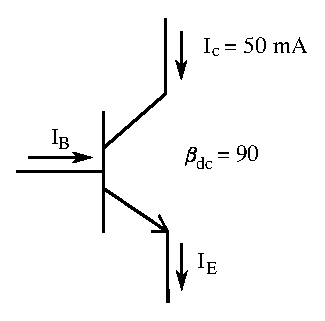
\includegraphics{chap2/fig7.eps}
\caption{}\label{fig2.7}
\end{figure}
\end{problem}

\eject

\begin{solution}
From given figure $\rmI_{\rmC}=50$~mA, \ $\beta_{\text{dc}}=90$

We have
\begin{align*}
\rmI_{\rmC} &\simeq \beta_{\text{dc}}\rmI_{\rmB}\\[4pt]
\therefore\quad \rmI_{\rmB} &\simeq \frac{\rmI_{\rmC}}{\beta_{\text{dc}}}=\dfrac{50\times 10^{-3}}{90}=555.5\mu\rmA\\[4pt]
\text{and}\quad \rmI_{\rmE} &= \rmI_{\rmC}+\rmI_{\rmB}\\[4pt]
&= 50\times 10^{-3}+555.5\times 10^{-6}\\[4pt]
\rmI_{\rmE} &= 50.55\text{~mA}
\end{align*}
\end{solution}

\begin{problem}\label{prob2.11}
Determine the value of $\rmI_{\rmC}$ and $\rmI_{\rmB}$ for the circuit shown in Fig.~\ref{fig2.8}. Neglect leakage current.
\begin{figure}[H]
\centering
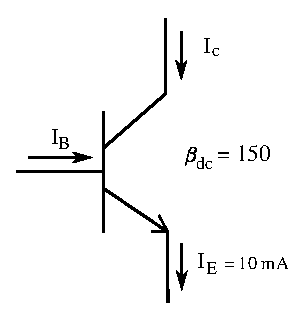
\includegraphics{chap2/fig8.eps}
\caption{}\label{fig2.8}
\end{figure}
\end{problem}

\begin{solution}
From give figure, $\rmI_{\rmE}=10\text{~mA}$, \ $\beta_{\text{dc}}=150$.

We have
\begin{align*}
\rmI_{\rmC} &= \beta_{\text{dc}}\rmI_{\rmB}\\[4pt]
(\rmI_{\rmE}-\rmI_{\rmB}) &= \beta_{\text{dc}}\rmI_{\rmB}\qquad [\because \ \rmI_{\rmE}=\rmI_{\rmC}+\rmI_{\rmB}]\\[4pt]
\rmI_{\rmB} &= \frac{\rmI_{\rmE}}{1+\beta_{\text{dc}}}\\[4pt]
&= \frac{10\times 10^{-3}}{1+150}\\[4pt]
\rmI_{\rmB} &= 66.23\mu\rmA\\[4pt]
\therefore\quad \rmI_{\rmC} &= \rmI_{\rmE}-\rmI_{\rmB}\\[2pt]
&= 10\times 10^{-3}-66.23\times 10^{-6}\\[2pt]
\rmI_{\rmC} &= 9.93\text{~mA}
\end{align*}
\end{solution}

\section{Transistor as an amplifier}\label{sec2.3}

Amplification is a process of increasing the amplitude of an electrical signal linearly and is one of the major properties of a transistor. When a transistor is biased in such a way that the emitter-base junction is forward biased and the collector-base junction is reverse biased, it is said to be in the {\em active region}. When a transistor is in the active region, the emitter-base junction has a low resistance and collector-base junction has a high resistance.

Before introducing the concept of amplification process, the designations that we used in this chapter for representing the circuit quantities of current, voltage and resistance must be explained because amplifier circuits have both dc and ac quantities. DC quantities are represented with an upper case subscript. For example $\rmI_{\rmB}$, $\rmI_{\rmE}$ and $\rmI_{\rmC}$ are the transistor dc currents. Similarly $\rmV_{\text{BE}}$, $\rmV_{\text{CB}}$ and $\rmV_{\text{CE}}$ are the dc voltages from transistor's one terminal to another. Single subscripted voltages such as $\rmV_{\rmB}$, $\rmV_{\rmC}$ and $\rmV_{\rmE}$ are dc voltages from the transistor terminals to the common point or ground.

AC quantities (time varying quantities) are represented with a lower case subscript. For example $\rmI_{\rmb}$, $\rmI_{\rme}$ and $\rmI_{\rmc}$ are the transistor ac currents. Similarly $\rmV_{\text{be}}$, $\rmV_{\text{ce}}$ and $\rmV_{\text{bc}}$ are the ac voltages from transistor's one terminal to another. Single subscripted voltages from the transistor terminals to the common point or ground.

Now, let us see how a transistor amplifies an electrical signal $\upsilon_{\text{in}}$. We know that, a transistor amplifies current because the collector current is equal to the base-current multiplied by the current gain $\beta_{\text{dc}}$ (i.e., $\rmI_{\rmC}=\beta_{\text{dc}}\rmI_{\rmB}$). The base current in a transistor is very small compared to the collector and emitter current.

Consider an ac voltage $\upsilon_{\text{in}}$ is superimposed on the dc bias voltage $\rmV_{\text{BB}}$ by connecting them in series with the base resistor $\rmR_{\rmS}$ as shown in Fig.~\ref{fig2.9}(a). The dc bias voltage $\rmV_{\text{CC}}$ is connected to the collector through the collector resistor $\rmR_{\rmC}$.

The superimposed ac input voltage $\rmV_{\text{in}}$ produces an ac base current, which results in a much larger ac collector current. This ac collector current produces an ac voltage across $\rmR_{\rmc}$, thus producing an amplified but inverted reproduction of the ac input voltage $\upsilon_{\text{in}}$ across $\rmR_{\rmc}$.

Fig.~\ref{fig2.9}(b) shows the ac equivalent circuit of the circuit shown in Fig.~\ref{fig2.9}(a). While writing an ac equivalent circuit all dc quantities are assumed to be zero. (i.e. $\rmV_{\text{BB}}$ and $\rmV_{\text{CC}}$ are zero). The forward biased emitter-base junction presents a very low resistance to the input ac signal.
\begin{figure}[H]
\centering
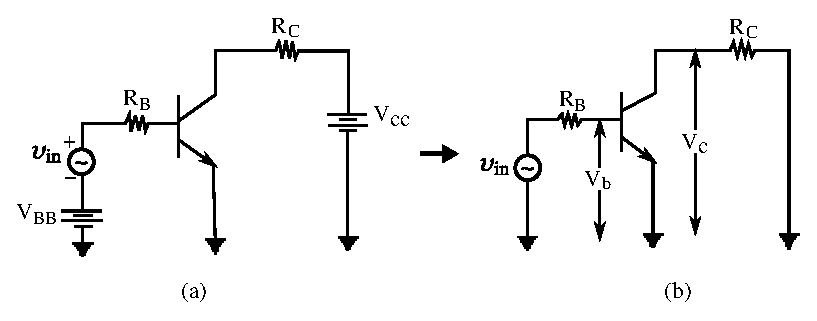
\includegraphics{chap2/fig9.eps}
\caption{(a) Circuit with an ac input voltage $\upsilon_{\text{in}}$ and dc bias voltage $\rmV_{\rmB\rmB}$ superimposed (b) AC equivalent circuit}\label{fig2.9}
\end{figure}

This internal ac emitter resistance is designated as $\rmr_{\rme}$ and is given by 
\begin{equation}
\rmr_{\rme} = \frac{\rmV_{\rmb}}{\rmI_{\rme}}\simeq \frac{\rmV_{\rmb}}{\rmI_{\rmc}}\qquad [\because ~~ \rmI_{\rme}\simeq \rmI_{\rmc}]\label{eq2.20}
\end{equation}

The ac collector voltage $\rmV_{\rmc}$ equal to the ac voltage drop across $\rmR_{\rmc}$.
\begin{equation}
\therefore\quad \rmV_{\rmc} = \rmI_{\rmc}\rmR_{\rmC}\label{eq2.21}
\end{equation}

Since $\rmI_{\rme}\simeq \rmI_{\rmc}$, the ac collector voltage is given by
\begin{equation}
\rmV_{\rmc}\simeq \rmI_{\rme}\rmR_{\rmC}\label{eq2.22}
\end{equation}

Consider $\rmV_{\rmb}$ as the transistor ac input voltage where, $\rmV_{\rmb}=\upsilon_{\text{in}}-\rmI_{\rmb}\rmR_{\rmB}$. $\rmV_{\rmC}$ can be considered as the transistor ac output voltage. Then the ratio of $\rmV_{\rme}$ to $\rmV_{\rmb}$ is the ac voltage gain $\rmA_{\nu}$ and is given by
\begin{equation}
\rmA_{\nu}=\frac{\rmV_{\rmc}}{\rmV_{\rmb}}\label{eq2.23}
\end{equation}
Also we have
\begin{equation}
\rmV_{\rmb}=\rmI_{\rme}\rmr_{\rme}\label{eq2.24}
\end{equation}

Substituting Eqns.~\eqref{eq2.22} and \eqref{eq2.24} in Eqn.~\eqref{eq2.23}, we get
\begin{align}
& \rmA_{\nu} = \frac{\rmV_{\rmc}}{\rmV_{\rmb}}\simeq \frac{\rmI_{\rme}\rmR_{\rmC}}{\rmI_{\rme}\rmr_{\rme}}\notag\\[3pt]
\therefore\quad & \text{AC voltage gain~~ } \rmA_{\nu}\simeq \frac{\rmR_{\rmC}}{\rmr_{\rme}}\label{eq2.25}
\end{align}

Since $\rmR_{\rmc}$ is always much greater than $\rmr_{\rme}$, the output voltage $\rmV_{\rme}$ is always greater than the input voltage $\rmV_{\rmb}$. Thus the transistor amplifies input electrical signal.

\begin{note}
Consider the basic transistor bias circuit configuration shown in Fig.~\ref{fig2.10} below. Three transistor dc currents ($\rmI_{\rmB}$, $\rmI_{\rmC}$ and $\rmI_{\rmE}$) and three dc voltages ($\rmV_{\text{BE}}$, $\rmV_{\text{CE}}$ and $\rmV_{\text{CB}}$) can be identified.

\smallskip 
\begin{figure}[H]
\centering
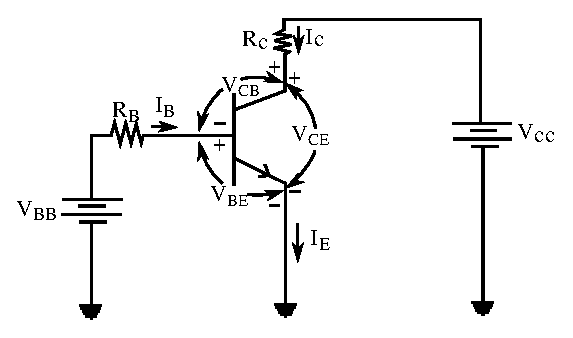
\includegraphics[scale=1.05]{chap2/fig10.eps}
\caption{Circuit showing the transistor with all dc currents and dc voltages}\label{fig2.10}
\end{figure}
\end{note}

\itheading{Introduction to Characteristics of transistors}
\medskip

So far we have discussed about the construction of a transistor and its current gain $\alpha_{\text{dc}}$ and $\beta_{\text{dc}}$. As a matter of fact, the value of $\alpha_{\text{dc}}$ and $\beta_{\text{dc}}$ do not completely explain the behaviour of a transistor. Many more details of a transistor can be studied with the help of curves, which relate the transistor currents and voltages. These curves are known as {\em characteristics} curves of transistor. Basically, there are two sets of characteristic curves for a transistor.
\begin{itemize}
\item[(i)] {\em Input characteristics}~: These curves give the relationship between input voltage and input current keeping output voltage constant.

\item[(ii)] {\em Output characteristics}~: These curves give the relationship between output voltage and output current keeping input current constant.
\end{itemize}

These two set of characteristics completely describe the operation of a transistor. Depending upon the configuration, the transistor characteristics may be mainly studied under the following two heads.
\begin{itemize}
\item[(i)] Characteristics of transistor in common-base (CB) configuration.

\item[(ii)] Characteristics of transistor in common-emitter (CE) configuration.
\end{itemize}

\newpage

\section{Common-Base Configuration}\label{sec2.4}

In this configuration, input is applied between the emitter and base junction and output is taken between collector and base junction. Hence base is common to both input and output.

\itheading{Characteristics in CB configuration}~: Following are two important characteristics of a transistor in common-base configuration.
\begin{itemize}
\item[(i)] {\em Input characteristics}~: These curves give the relationship between the emitter current and the emitter-base junction voltage for a constant collector-base junction voltage.

\item[(ii)] {\em Output characteristics}~: These curves give the relationship between the collector current and the collector-base junction voltage for a constant emitter current.
\end{itemize}

These characteristics for an npn transistor may be obtained using a circuit as shown in Fig.~\ref{fig2.11}.
\begin{figure}[H]
\centering
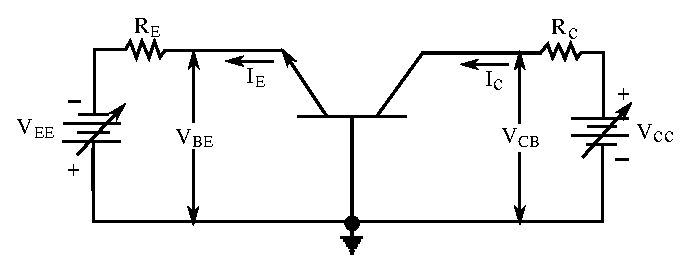
\includegraphics{chap2/fig11.eps}
\caption{Circuit arrangement to determine the characteristics of an npn transistor in CB configuration}\label{fig2.11}
\end{figure}

In this circuit, an npn transistor is connected in common-base configuration. The emitter-to-base voltage $\rmV_{\text{BE}}$ can be varied by varying the dc supply $\rmV_{\text{EE}}$ and the collector-to-base voltage $\rmV_{\text{CB}}$ can be varied by varying the dc supply $\rmV_{\text{CC}}$. 

The dc milli-ammeters and dc voltmeters connected in the emitter and collector circuits of the transistor to measure the currents and voltages are not shown for simplicity.

\heading{Input Characteristics}~: These characteristics may be obtained by using the circuit shown in Fig.~\ref{fig2.11} as explained below. Firstly, adjust the collector-to-base voltage $\rmV_{\text{CB}}$ to zero volt. Then increase the emitter-to-base voltage $\rmV_{\text{BE}}$ in small suitable steps (say in steps of 0.05 V) and note down the corresponding values of emitter current $\rmI_{\rmE}$ at each step. Now, if we plot a graph with emitter-to-base voltage $\rmV_{\text{EB}}$ along the horizontal axis and the emitter current $\rmI_{\rmE}$ along the vertical axis, we will obtain a curve marked $\rmV_{\text{CB}}=0\rmV$ as shown in Fig.~\ref{fig2.12} below. A similar procedure may be repeated to obtain curves at different collector-to-base voltages (say $\rmV_{\text{CB}}=4\rmV$, $\rmV_{\text{CB}}=8\rmV$ etc.) as shown in Fig.~\ref{fig2.12}.

\smallskip
\begin{figure}[H]
\centering
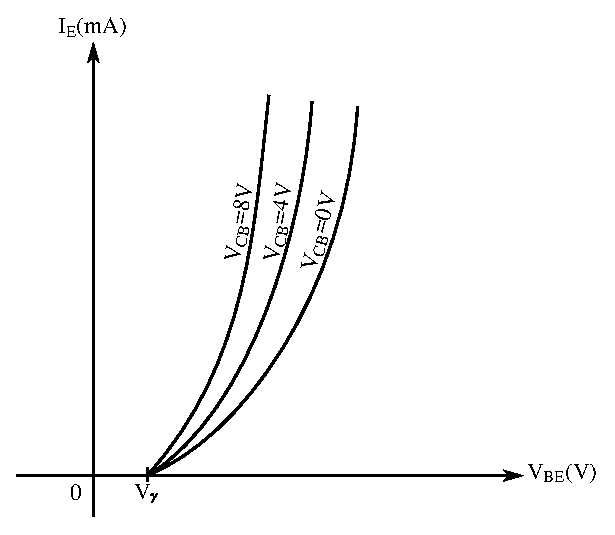
\includegraphics{chap2/fig12.eps}
\caption{Input characteristics of an npn transistor in CB configuration}\label{fig2.12}
\end{figure}

\smallskip
It will be interesting to know that the input characteristics give us the following important informations.
\begin{itemize}
\item[(a)] There exist a cut-in voltage or knee voltage $\rmV_{\gamma}$ below which the emitter current $\rmI_{\rmE}$ is negligibly small. The value of cut-in voltage $\rmV_{\gamma}$ is approximately 0.6 V for Si and 0.2 V for Ge transistors.

\item[(b)] Beyond cut-in voltage $\rmV_{\gamma}$, for a fixed collector-to-base voltage $\rmV_{\text{CB}}$, the emitter current $\rmI_{\rmE}$ increases rapidly with a small increase in emitter-to-base voltage $\rmV_{\text{BE}}$. It means that input resistance of a transistor in common-base configuration is very small.

\item[(c)] As the collector-to-base voltage $\rmV_{\text{CB}}$ increases, the input characteristics curves shift inward.
\end{itemize}

\newpage

\heading{Output Characteristics~:} These characteristics may be obtained by using the circuit shown in Fig.~\ref{fig2.11} as explained below. Firstly, we adjust the emitter to base voltage $\rmV_{\text{BE}}$ to get a suitable value of an emitter current (say 1 mA). Keeping the emitter current $\rmI_{\rmE}$ constant, we increase the collector-to-base voltage $\rmV_{\text{CB}}$ from lowest value in a number of suitable steps and note down the corresponding values of the collector current $\rmI_{\rmC}$ at each step. If we plot a graph with collector-to-base voltage $\rmV_{\text{CB}}$ along the horizontal axis and the collector current $\rmI_{\rmC}$ along the vertical axis, we will obtain a curve marked $\rmI_{\rmE}=1$~mA as shown in Fig.~\ref{fig2.13}. A similar procedure may be repeated to obtain the characteristics for different values of emitter current (say $\rmI_{\rmE}=3$~mA, $\rmI_{\rmE}=5$~mA etc.)
\begin{figure}[H]
\centering
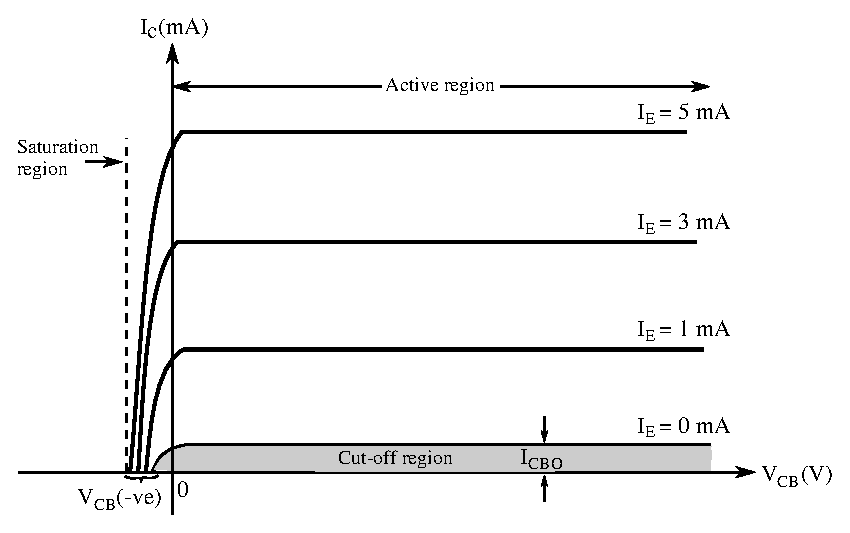
\includegraphics{chap2/fig13.eps}
\caption{Output characteristics of an npn transistor in CB configuration}\label{fig2.13}
\end{figure}

The output characteristics gives the following important informations.
\begin{itemize}
\item[(a)] The characteristics may be divided into 3 regions namely saturation region, active region and cut-off region. The saturation region is the region to the left of the $\rmV_{\text{CB}}=0$ axis. It may be noted that in this region, collector-to-base voltage $\rmV_{\text{CB}}$ is negative for an npn transistor. It means that collector-to-base junction is also forward biased in the saturation region. In this region a small change in $\rmV_{\text{CB}}$ results in a large change in $\rmI_{\rmC}$. The active region is the region right to the $\rmV_{\text{CB}}=0$ axis and above $\rmI_{\rmE}=0$ curve. In the active region, the collector current $\rmI_{\rmC}$ is constant and is almost, equal to the emitter current $\rmI_{\rmE}$. The cut-off region is the region below $\rmI_{\rmE}=0$ curve, which is shown by a shaded region in Fig.~\ref{fig2.13}. In the cut-off region both the junctions are reverse biased.

\item[(b)] The collector current $\rmI_{\rmC}$ flows even when the collector-to-base voltage $\rmV_{\text{CB}}$ is zero.

\item[(c)] A small collector current $\rmI_{\rmC}=\rmI_{\text{CBO}}$ flows even when emitter current $\rmI_{\rmE}$ is zero. This current is called collector-to-base leakage current $\rmI_{\text{CBO}}$.

\item[(d)] The collector current $\rmI_{\rmC}$ is independent of collector-to-base voltage $\rmV_{\text{CB}}$ in the active region.

\item[(e)] The output characteristic curves of a transistor in common-base configuration are almost horizontal which indicates that the value of output resistance is very high.
\end{itemize}

\section{Common-Emitter Configuration}\label{sec2.5}

In this configuration input is applied between base and emitter and output is taken between collector and emitter. Hence the emitter is common to both input and output.

\itheading{Characteristics in CE configuration~:} Following are the two important characteristics of a transistor in common-emitter configuration.
\begin{itemize}
\item[(i)] {\em Input characteristics~:} These curves give the relationship between the base current and the base-to-emitter voltage for a constant collector-to-emitter voltage.

\item[(ii)] {\em Output characteristics~:} These curves give the relationship between the collector current and the collector-to-emitter voltage for a constant base current.
\end{itemize}

These characteristics may be obtained using a circuit as shown in Fig.~\ref{fig2.14}.

\smallskip
In this circuit, an npn transistor is connected in common-emitter configuration. The base-to-emitter voltage $\rmV_{\text{BE}}$ can be varied by varying the dc supply $\rmV_{\text{BB}}$ and the collector-to-emitter voltage $\rmV_{\text{CE}}$ can be varied by varying the dc supply $\rmV_{\text{CC}}$. The dc micro-ammetor to measure $\rmI_{\rmB}$, dc milli-ammeter to measure $\rmI_{\rmC}$ and dc voltmeters to measure voltages $\rmV_{\text{BE}}$ and $\rmV_{\text{CE}}$ are not shown for simplicity.
\begin{figure}[H]
\centering
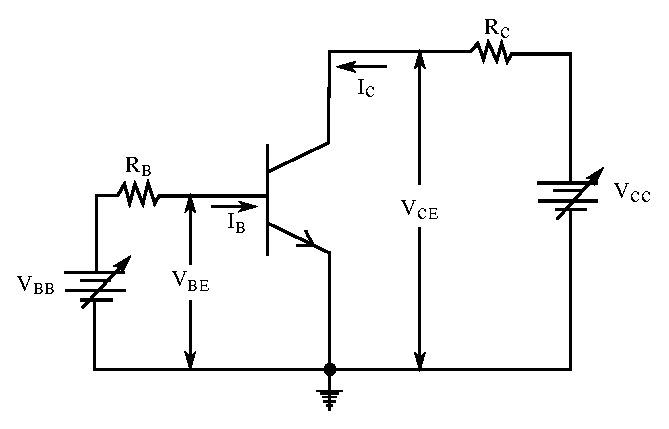
\includegraphics{chap2/fig14.eps}
\smallskip
\caption{Circuit arrangement to determine the characteristics of an npn transistor in CE configuration}\label{fig2.14}
\end{figure}

\heading{Input Characteristics~:} These characteristics may be obtained by using the circuit shown in Fig.~\ref{fig2.14} as explained below. Firstly, adjust the collector-to-emitter voltage $\rmV_{\text{CE}}$ to zero volts. Then increase the base-to-emitter voltage $\rmV_{\text{BE}}$ in small suitable steps (say in steps of 0.05 V) and note down the corresponding values of base current $\rmI_{\rmB}$ at each step. Now, if we plot a graph with base-to-emitter voltage $\rmV_{\text{BE}}$ along the horizontal axis and the base current $\rmI_{\rmB}$ along the vertical axis, we will obtain a curve marked with $\rmV_{\text{CE}}=0\rmV$ as shown in Fig.~\ref{fig2.15} below. A similar procedure may be repeated to obtain curves for different collector-to-emitter voltages (say $\rmV_{\text{CE}}=3\rmV$, $\rmV_{\text{CE}}=6\rmV$ etc.) as shown in the Fig.~\ref{fig2.15}.

It will be interesting to know that the input characteristics give us the following informatitions.
\begin{itemize}
\itemsep=0pt
\item[(a)] There exist a cut-in voltage or knee voltage $\rmV_{\gamma}$ below which the base current $\rmI_{\rmB}$ is negligibly small. The value of cut-in voltage $\rmV_{\gamma}$ is approximately 0.6\,V for Si and 0.2 V for Ge transistors.

\item[(b)] Beyond cut-in voltage $\rmV_{\gamma}$, for a fixed collector-to-emitter voltage $\rmV_{\text{CE}}$, the base current $\rmI_{\rmB}$ increases rapidly with a increase in base-to-emitter voltage $\rmV_{\text{BE}}$. But the base current $\rmI_{\rmB}$ does not increase as rapidly as that of input characteristics of a common-base configuration. Therefore, the input resistance of a transistor in common-emitter configuration in higher as compared to common-base configuration.

\item[(c)] As the collector-to-emitter voltage $\rmV_{\text{CE}}$ increases, the input characteristic curves shift outward.
\end{itemize}
\begin{figure}[H]
\centering
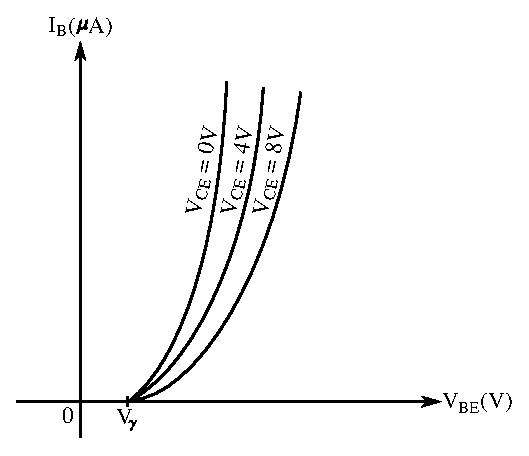
\includegraphics{chap2/fig15.eps}

\smallskip
\caption{Input characteristics of an npn transistor in CE configuration}\label{fig2.15}
\end{figure}

\heading{Output characteristics~:} These characteristics may be obtained by using the circuit shown in Fig.~\ref{fig2.15} as explained below. Firstly, we adjust the base-to-emitter voltage $\rmV_{\text{BE}}$ to get a suitable value of base current $\rmI_{\rmB}$. (say $5\mu\rmA$). Keeping the base current $\rmI_{\rmB}$ constant, we increase the collector-to-emitter voltage $\rmV_{\text{CE}}$ from zero in a number of suitable steps and note down the corresponding values of collector current $\rmI_{\rmC}$ at each step. If we plot a graph with collector-to-emitter voltage $\rmV_{\text{CE}}$ along the horizontal axis and collector current $\rmI_{\rmC}$ along the vertical axis, we will obtain a curve marked $\rmI_{\rmB}=5\mu\rmA$, as shown in Fig.~\ref{fig2.16}. A similar procedure may be repeated to obtain the characteristics at different values of base current $\rmI_{\rmB}$. (say $\rmI_{\rmB}=10\mu\rmA$, $\rmI_{\rmB}=15\mu\rmA$ etc.).

\smallskip
The output characteristics give the following important informations.
\begin{itemize}
\item[(a)] The output characteristics may be divided into three important regions, namely, saturation region, active region and cut-off region. The saturation and cut-off regions are shown by the shaded areas, whereas the active region is the region between saturation and cut-off regions.

\newpage

\item[(b)] As the collector-to-emitter voltage $\rmV_{\text{CE}}$ is increased above zero, the collector current $\rmI_{\rmC}$ increases rapidly to a saturation value, depending upon the value of base current $\rmI_{\rmB}$. Generally, the collector current $\rmI_{\rmC}$ reaches to a saturation value when $\rmV_{\text{CE}}$ is about 0.3\,V.

\item[(c)] When collector-to-emitter voltage is increased in the active region, the collector current $\rmI_{\rmC}$ increases slightly.

\item[(d)] When the base current is zero, a small collector current $\rmI_{\rmC}=\rmI_{\text{CO}}=(\beta_{\text{dc}}+1)\rmI_{\text{CBO}}$ exists as shown in Fig.~\ref{fig2.16}. This is called {\em leakage current}, which is negligibly small. Under this condition, the transistor is at cut-off.
\end{itemize}
\begin{figure}[H]
\centering
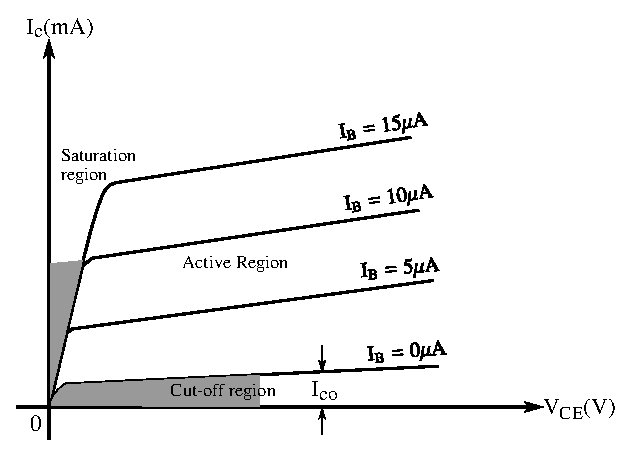
\includegraphics{chap2/fig16.eps}
\caption{Output characteristics of an npn transistor in CE configuration}\label{fig2.16}
\end{figure}



\subsection{CE cut-off region}\label{sec2.5.1}

As already explained, when $\rmI_{\rmB}=0$, the transistor is in the cut-off region of its operation. This is shown in Fig.~\ref{fig2.17} below, with the base load open, resulting in a base current of zero.

\smallskip
When the transistor is in cut-off region, there exist a very small amount of collector leakage current $\rmI_{\text{CO}}$. This is mainly due to thermally generated charge carriers. Since $\rmI_{\text{CO}}$ is extremely small, it is usually neglected in the circuit analysis, so that $\rmV_{\text{CE}}\simeq \rmV_{\text{CC}}$. In cut-off region, both the emitter-base and the collector-base junctions are reverse biased.
\begin{figure}[H]
\centering
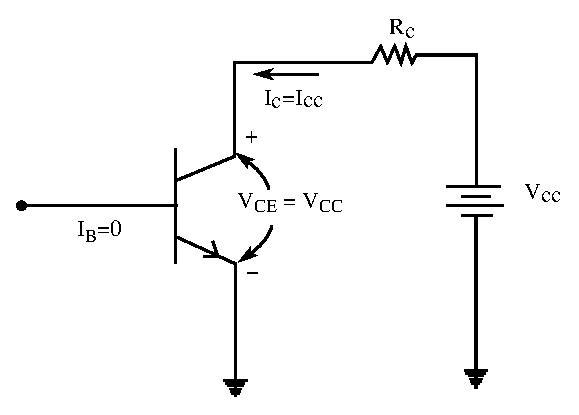
\includegraphics{chap2/fig17.eps}
\smallskip
\caption{Transistor in cut-off region}\label{fig2.17}
\end{figure}

\smallskip
\subsection{CE Saturation region}\label{sec2.5.2}

Consider the circuit shown in Fig.~\ref{fig2.18} below.
\begin{figure}[H]
\centering
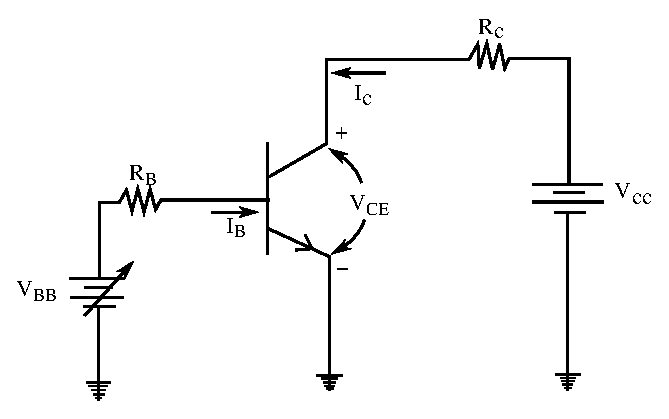
\includegraphics{chap2/fig18.eps}
\smallskip
\caption{Circuit to illustrate saturation region}\label{fig2.18}
\end{figure}

\eject

When the emitter-base junction is forward biased and the base current $\rmI_{\rmB}$ is increased, the collector current $\rmI_{\rmC}$ also increases ($\because ~ \rmI_{\rmC}=\beta_{\text{dc}}\rmI_{\rmB}$) and $\rmV_{\text{CE}}$ decreases, as a result of more voltage drop across the collector resistor $\rmR_{\rmC}$.
$$
\because\quad \rmV_{\text{CE}}=\rmV_{\text{CC}}-\rmI_{\rmC}\rmR_{\rmC}
$$

When $\rmV_{\text{CE}}$ reaches its saturation value $\rmV_{\text{CE(sat)}}$, the collector-base junction is forward biased and collector current $\rmI_{\rmC}$ cannot increase further even with a continued increase in base current $\rmI_{\rmB}$. At the point of saturation, the relation $\rmI_{\rmC}=\beta_{\text{dc}}\rmI_{\rmB}$ is no longer valid.

$\rmV_{\text{CE(sat)}}$ for a transistor occurs somewhere below the knee of common-emitter characteristics and it is usually few tenths of volts. In saturation region, both emitter-base and collector-base junctions are forward biased.

\section{DC and small-signal current gain}\label{sec2.6}

Consider the output characteristics of a transistor shown in Fig.~\ref{fig2.19}.
\begin{figure}[H]
\centering
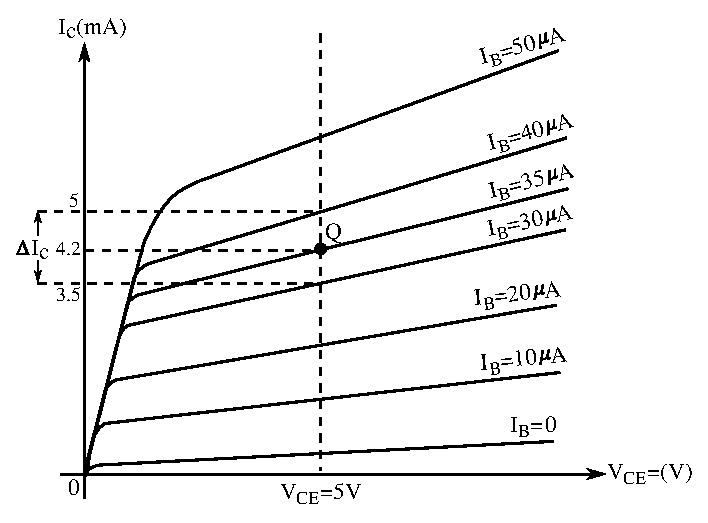
\includegraphics{chap2/fig19.eps}
\caption{Output characteristics of a transistor}\label{fig2.19}
\end{figure}

As we have already discussed, the ratio of dc collector current to dc base current is known as {\em dc current gain} of the transistor. It is denoted by $\beta_{\text{dc}}$. To find the value of $\beta_{\text{dc}}$, select a point $\rmQ$ in the active region of the transistor, as shown in Fig.~\ref{fig2.19}, and find the ratio of $\rmI_{\rmC}$ to $\rmI_{\rmB}$. For a given point $\rmQ$ in the Fig.~\ref{fig2.19}, it is found that, $\rmI_{\rmB}=35\mu\rmA$ and corresponding $\rmI_{\rmC}=4.2\text{~mA}$. Therefore, $\beta_{\text{dc}}$ at the point $\rmQ$ is,
$$
\beta_{\text{dc}}=\dfrac{\rmI_{\rmC}}{\rmI_{\rmB}}=\dfrac{4.2\times 10^{-3}}{35\times 10^{-6}}=120
$$

Even though the value of $\beta_{\text{dc}}$ varies by a small amount from point to point in the active region, it may be considered as almost constant for small signal operation.

The small signal current gain $\beta_{\text{ac}}$ is defined as the ratio of small change in collector current $\Delta \rmI_{\rmC}$ to small change in base current $\Delta\rmI_{\rmB}$, keeping $\rmV_{\text{CE}}$ constant.
\begin{equation}
\text{i.e.,}\qquad \beta_{\text{ac}}=\left.\dfrac{\Delta \rmI_{\rmC}}{\Delta \rmI_{\rmB}}\right|_{\rmV_{\text{CE}}=\text{constant}}\label{eq2.26}
\end{equation}

Evaluating this from Fig.~\ref{fig??}, for $\rmV_{\text{CE}}=5\rmV$, we get
\begin{align*}
\beta_{\text{ac}}=\left.\dfrac{\Delta \rmI_{\rmC}}{\Delta \rmI_{\rmB}}\right|=\dfrac{(5-3.5)\times 10^{-3}}{(40-30)\times 10^{-6}}=150\\[4pt]
\rmV_{\text{CE}} &= 5\rmV
\end{align*}
Generally $\beta_{\text{dc}}$ and $\beta_{\text{ac}}$ are almost equal.

\medskip

\begin{center}
\rule{4cm}{1pt}\\
{\bf\Large Problems}\\[-3pt]
\rule{4cm}{1pt}
\end{center}

\begin{problem}\label{prob2.12}
A transistor has its collector current increased from 15 to 20 mA, when the base current is increased from $320\mu\rmA$ to $480\mu\rmA$ keeping $\rmV_{\text{CE}}$ constant. Calculate $\beta_{\text{ac}}$ and $\alpha_{\text{ac}}$.
\end{problem}

\begin{solution}
We have $\Delta \rmI_{\rmC}=(20-15)\text{\,mA}=5\text{\,mA}$ \ and  \ $\Delta \rmI_{\rmB}=(480-320)\mu\rmA=160\mu\rmA$
\begin{align*}
\therefore\quad \beta_{\text{ac}} &= \left.\dfrac{\Delta \rmI_{\rmC}}{\Delta \rmI_{\rmB}}\right|_{\rmV_{\text{CE}}=\text{\,constant}}=\dfrac{5\times 10^{-3}}{160\times 10^{-6}}\simeq 31\\[4pt]
\therefore\quad \alpha_{\text{ac}} &= \frac{\beta_{\text{ac}}}{1+\beta_{\text{ac}}}=\dfrac{31}{1+31}=0.969
\end{align*}
\end{solution}

\eject

\begin{problem}\label{prob2.13}
The output characteristics of a transistor is shown in Fig.~\ref{fig2.20}. Determine $\beta_{\text{dc}}$, $\alpha_{\text{dc}}$, $\beta_{\text{ac}}$ and $\alpha_{\text{ac}}$ at point $\rmQ$ shown.
\begin{figure}[H]
\centering
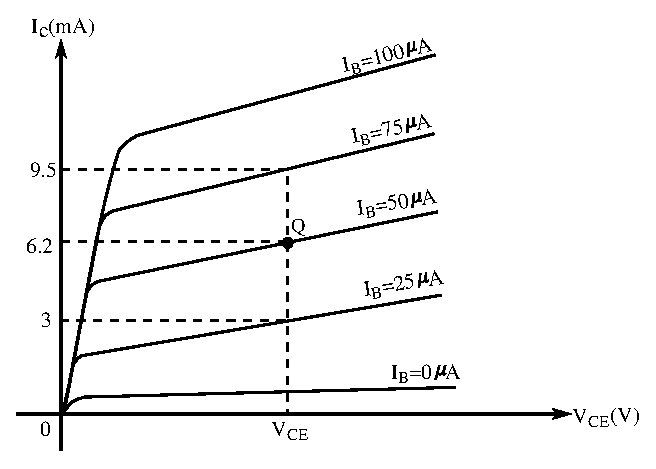
\includegraphics{chap2/fig20.eps}
\caption{}\label{fig2.20}
\end{figure}
\end{problem}










\label{2end}
